%--------------------------------------------------------------------
\medskip
\section{Mapas de influencia}
\label{mapas-influencia}
Los mapas de influencia reflejan la presencia o \textit{poder} de cada uno de los equipos en una zona o casilla concreta del mapa. Para cada personaje del equipo, la influencia del ese equipo comenzará desde la casilla actual en la que se encuentra el personaje y podrá extenderse una determinada distancia (una cantidad determinada de casillas alrededor del personaje). Aunque, es habitual que conforme mayor sea la distancia menor sea la influencia que ese personaje va teniendo sobre el terreno. \\

Tal y como hemos planteado los mapas de influencia, cada equipo tendrá su propio mapa de influencia y el contenido de cada uno de esos mapas se calculará en función de la posición de los personajes de ese equipo (solamente los de ese equipo). Esta separación inicial en diversos mapas nos servirá para disponer y controlar de una forma más exhaustiva la presencia y valores concretos de cada uno de los personajes de cada equipo. Cuando vayamos a dibujar la influencia final sobre el terreno, sí que tendrán en cuenta todos los mapas de todos los equipos. Es importante tener en cuenta que, aunque cada equipo tenga su propio mapa, \textbf{el equipo con mayor influencia en una casilla, controlará dicha casilla} (esto se tendrá en cuenta al dibujar el mapa). \\

A la hora de calcular la influencia que ejerce un personaje concreto sobre el terreno que le rodea, son necesarios 2 valores: el máximo valor de influencia (que será la influencia que se ejercerá sobre la casilla en la que se encuentra el personaje) y la máxima distancia de influencia (a partir de esa distancia, el personaje no ejercerá influencia sobre el terreno). Conforme nos vamos alejando de la casilla actual en la que se encuentra el personaje, \textbf{el valor de influencia va disminuyendo en 1}. El mecanismo de cálculo es la distancia de Chebyshev (tal y como se ha visto en la parte de pathfinding, aunque con algunas modificaciones). Teniendo en cuenta cual es el resultado de esta distancia, hemos considerado que aplicarla en este caso es la mejor opción y lo más conveniente. A la hora de modificar con la matriz de influencia de un equipo, solo se tendrá en cuenta la región afectada por un personaje concreto (de acuerdo a la distancia máxima establecida), es decir, que para cada personaje no se recorrerá la matriz entera. Cabe destacar que un personaje neutral no ejercerá influencia, no tendrá ninguna matriz asociada y no podrá tener acceso a esta funcionalidad. \\

Cuando hay varios personajes del mismo equipo cerca, a la hora de calcular el mapa de influencia de ese equipo, puede ocurrir que en valor de una celda supere el valor máximo permitido (ya que las influencias individuales se van sumando). Cuando esto ocurre simplemente sustituimos dicho valor por el máximo permitido. \\ 

Esta funcionalidad consta básicamente de los siguientes métodos:
\begin{itemize}
	\item En primer lugar, deberemos inicializar todas las variable necesarias usando los métodos habilitados para ello. Esto solo e hace 1 vez.
	\item A continuación, en cada iteración del bucle del juego debemos llamar al método \texttt{updateSimpleMapOfInfluence} para actualizar la información de los mapas de influencia. Cabe destacar que solamente se tendrán en cuenta los personajes como tal y no los objetos de tipo formación.
	\item Finalmente, debemos llamar al método de dibujo para poder visualizar la influencia que ejerce cada equipo sobre el terreno. O bien en forma de mini mapa o bien sobre el propio mapa completo (en función de los parámetro que pasemos a la función).	
\end{itemize}

Para realizar el dibujo del mapa de influencia calculado, existe el método \texttt{drawInfluenceMap}. Este método recibe los siguientes parámetros:
\begin{itemize}
	\item renderer.
	\item output\_grid\_cell\_size $\rightarrow$ Tamaño del lado de cada cuadradito o celda del mapa de influencia.
	\item positionX y positionY $\rightarrow$ Posición de la esquina inferior izquierda del mapa de influencia.
	\item filled $\rightarrow$ Booleano que indica si las celdas del mapa de influencia se rellenarán o no. Si este flag es falso, solamente se colorearán los lados de las celdas.
\end{itemize}

Ajustando el tamaño de celda y las posiciones de mapa podemos conseguir que el mapa de influencia se muestra como un minimapa junto al mapa real o sobre el propio mapa real (con los cuadrados no rellenos, en este caso). \\

A la hora de dibujar el mapa, cada equipo tiene distintos tonos de azul y distintos tonos de rojo (un equipo es el color azul y otro es el rojo). Además, el color banco representará una casilla neutral. Para cada posición del mapa de influencia, a parte de comprobar si la celda debe rellenarse/colorearse o no, también se harán otras comprobaciones:
\begin{itemize}
	\item Si el mapa de costes de terreno en esa posición corresponde con un terreno infranqueable, no se dibujará la influencia.
	\item Si la influencia de un equipo es mayor a la del otro, se dibujará del color correspondiente al equipo con mayor influencia y del tono de color correspondiente. Para obtener el todo de color correspondiente \textbf{se resta el valor del equipo con mayor influencia menos el valor del equipo con menor influencia} (puesto que aunque un equipo controle una casilla, la influencia del otro equipo también afecta). Ese resultado se divide entre 5 (porque hay 5 tonos de color por cada equipo) y se usa el tono correspondiente al cociente obtenido.
	\item Finalmente, si el parámetro \texttt{filled} está a true. Se dibuja la celda de color blanco. Esto se usa para que, en el caso del minimapa, sí aparenza el fondo blanco, pero en el caso de dibujar el mapa de influencia sobre el mapa real, solamente aparezcan las influencias de los equipos y no se dibujen las zonas sin influencia.
\end{itemize}

A la hora de integran esta información con el pathfinding táctico de un personaje, habría que pasar el mapa de influencia \textbf{del equipo contrario}. El pathfinding debe tener en cuenta la influencia del equipo rival (coste añadido) para NO IR por esas zonas. Por tanto, a priori no tiene sentido usar el mapa de influencia de mi propio equipo, ya que estaría penalizando las zonas controladas por mí. \\

Para finalizar, voy a adjuntar una captura de pantalla de nuestro videojuego en la que se puede observar el mapa de influencia final dibujado (tanto en forma de minimapa como sobre el mapa real):
\begin{figure}[!th]
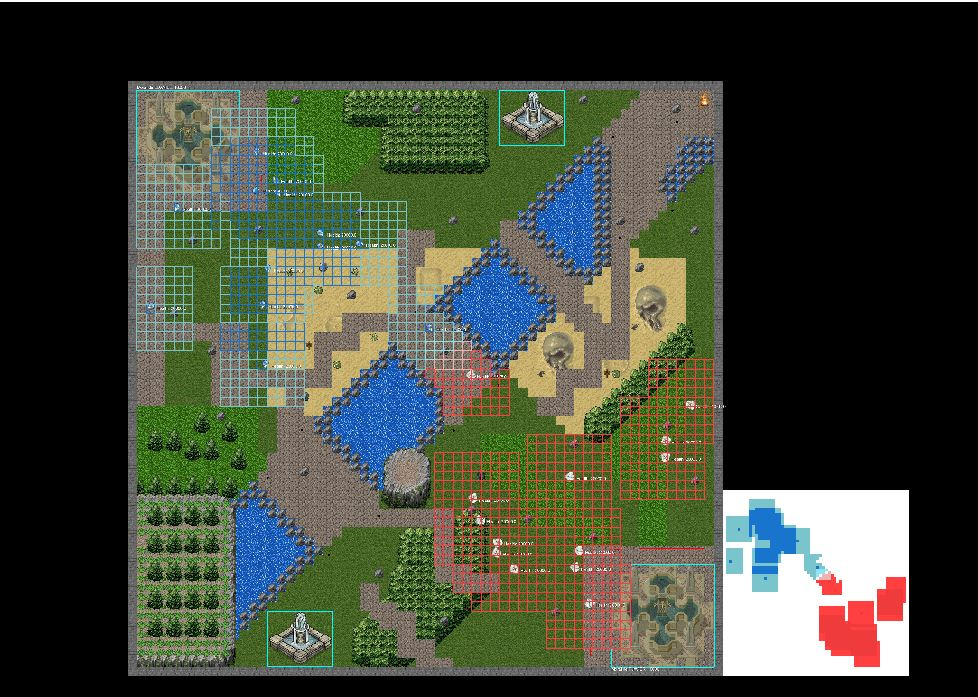
\includegraphics[scale=0.6]{influencia}
\centering
\caption{Mapa de influencia.}
\label{mapa:mapa}
\end{figure}